\section{The History of Gamma-ray Astrophysics}
\seclabel{history_gamma_ray_detectors}

It was only natural to wonder about photons with even
higher energies. 
As is common in the field of physics, the prediction of
the detection of cosmic $\gamma$-rays proceeded their discovery.
\cite{feenberg_1948_interaction-cosmic-ray} theorized that the interaction
of starlight with cosmic rays could produce $\gamma$-rays through
\ac{IC} upscattering.  Following the discovery of the neutral
pion in 1949, \cite{hayakawa_1952_propagation-cosmic}
predicted that $\gamma$-ray emission could be observed from the
decay of neutral pions when cosmic rays interacted with interstellar
matter.  And in the same year, \cite{hutchinson_1952_possible-relation}
discussed the bremsstrahlung radiation of cosmic-ray electrons.
\cite{morrison_1958_gamma-ray-astronomy} predicted the detectability
of $\gamma$-ray emission from solar flares, \acp{PWN}, and active galaxies.

The first space-based $\gamma$-ray detector was \explorerxi
\citep{kraushaar_1965_explorer-experiment}.  \explorerxi operated in
the energy energy range above $100\unitspace\mev$.  It had an area of
$\sim45\cm^2$ but an effective area of only $\sim 7\cm^2$, corresponding
to a detector efficiency of $\sim 15\%$.  It was launched on April
27, 1961 and was in operation for 7 months.  \explorerxi observed 31
$\gamma$-rays but, because the distribution a distribution of these
$\gamma$-rays was consistent isotropy, the experiment could not firmly
identify the $\gamma$-rays as being cosmic.

The first definitive detection of $\gamma$-ray came in
1962 by an experiment on the Ranger 3 moon
probe \citep{arnold_1962_gamma-space}.  It detected an isotropic flux
of $\gamma$-rays in the 0.5 \mev to 2.1 \mev energy range.

\Ac{OSO-3} was the first experiment to firmly identify
$\gamma$-ray emission from the Galaxy
\citep{kraushaar_1972_high-energy-cosmic}.  
\Ac{OSO-3} was launched on March 8, 1967 and operated for 16 months, measuring
621 cosmic $\gamma$-rays.  
\figref{oso3_skymap} shows a sky map of these $\gamma$-rays.  This
experiment confirmed both a Galactic component to the $\gamma$-ray
sky as well as an additional isotropic component, hypothesised to be
extragalactic in origin.

\begin{figure}[htbp]
  \centering
  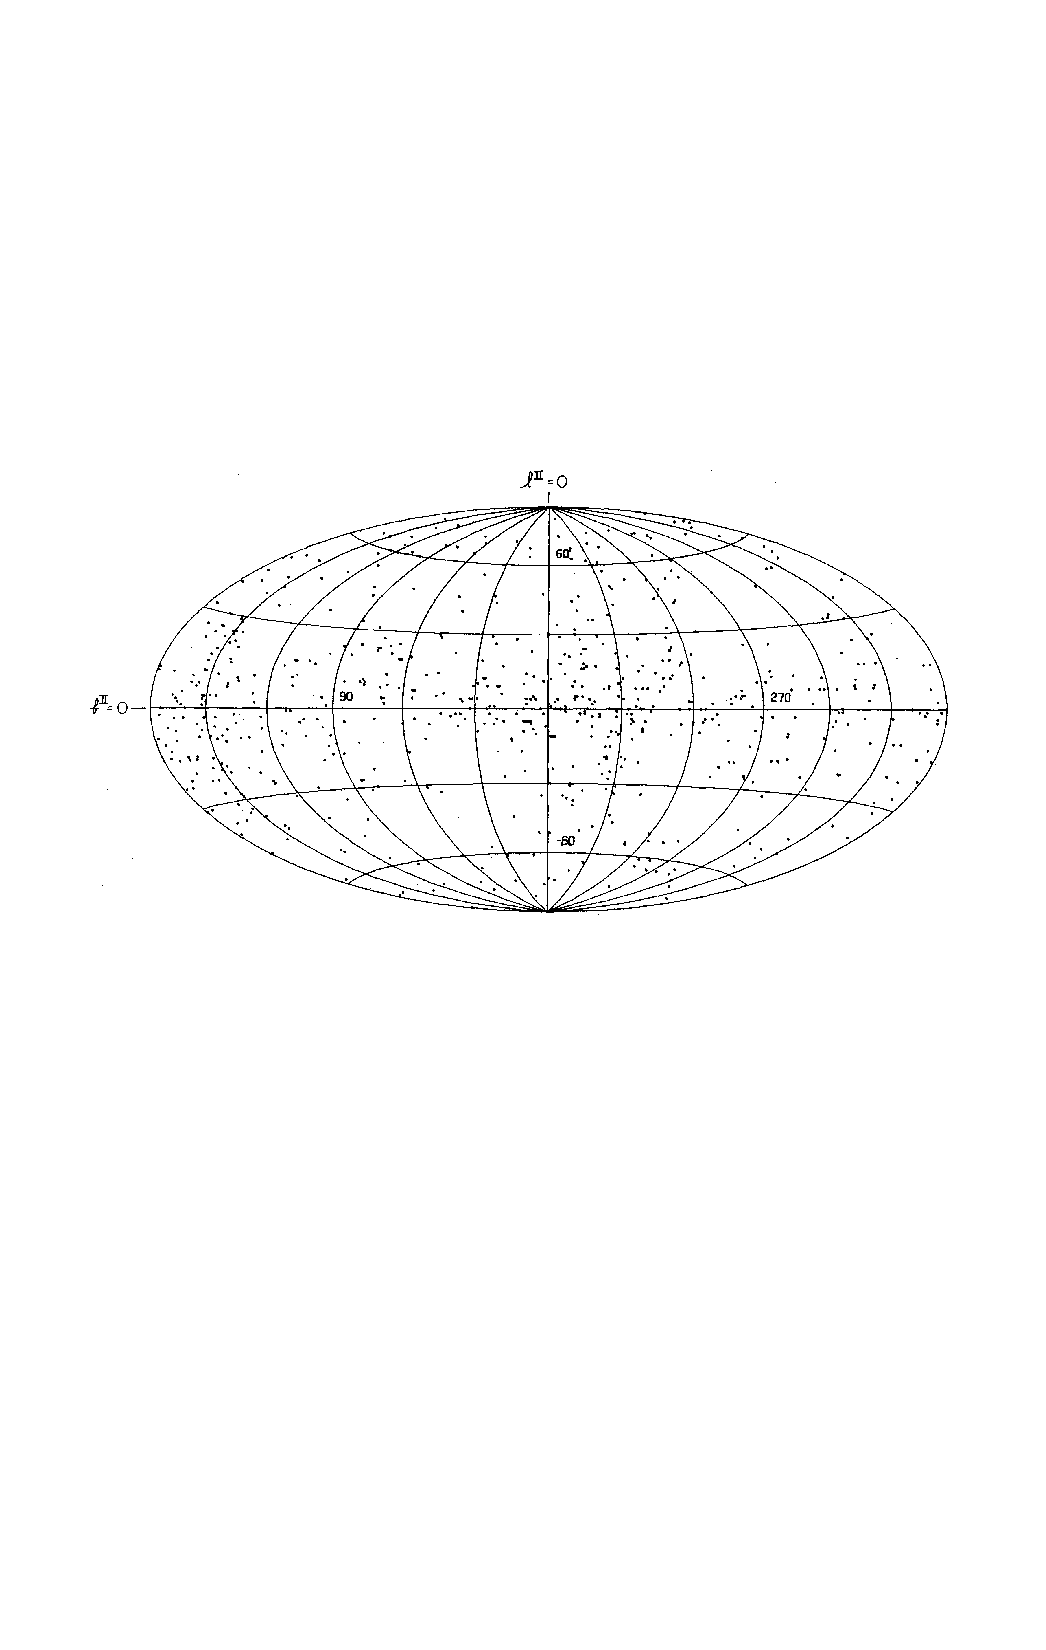
\includegraphics{chapters/introduction/figures/kraushaar_et_al_1972_skymap.pdf}
  \figlabel{oso3_skymap}
  \caption{The position of all 621 cosmic $\gamma$-rays
  detected by \ac{OSO-3}. This figure is from
  \cite{kraushaar_1972_high-energy-cosmic}. }
\end{figure}

This anisotropic $gamma$-ray distribution
was confirmed by a balloon-based
$\gamma$-ray detector in 1970  \citep{kniffen_1970_study-gamma}.  In the
following year, the first $\gamma$-ray pulsar (the Crab pulsar) was detected
by another balloon-based detector \cite{browning_1971_detection-pulsed}.

The next major advancements in $\gamma$-ray astronomy
came from \ac{SAS-2} and \cosb.  \Ac{SAS-2} was a dedicated
$\gamma$-ray detector launched by \ac{NASA} in November 15, 1972
\cite{fichtel_1975_high-energy-gamma-ray}. It improved upon \ac{OSO-3}
by incorporating a spark chamber and having an overall larger size.
The size of the active area of the detector was 640 $\cm^2$ and the
experiment had a much improved effective area of $\sim 115\unitspace
cm^2$. The spark chamber allowed for a separate measurement of the
electron and positron tracks, which allowed for improved directional
reconstruction of the incident $\gamma$-rays. \Ac{SAS-2} had a PSF
$\sim5\degree$ at 30 \mev and $\sim1\degree$ at 1 \gev.

In 6 months, \ac{SAS-2} observed over 8,000 $\gamma$-ray
photons and covered $\sim55\%$ of the sky including most of
the Galactic plane.  It discovered pulsations from the Crab
\citep{fichtel_1975_high-energy-gamma-ray} and Vela pulsar
\citep{thompson_1977_sas-2-high-energy}.  In addition, \ac{SAS-2}
discovered Geminga, the first $\gamma$-ray source with no compelling
multiwavelength counterpart \citep{thompson_1977_final-sas-2}. Geminga
was eventually discovered to be a pulsar by \ac{EGRET}
\citep{bertsch_1992_pulsed-high-energy} and retroactively by \ac{SAS-2}
\citep{mattox_1992_observation-pulsed}.

\ac{ESA} launched \cosb on August 9, 1975.
\cosb improved upon
the design of \ac{SAS-2} by including a calorimeter below the spark
chamber which improved the energy resolution to $<100\%$ for energies
$\sim 3\unitspace\gev$ \citep{bignami_1975_cos-b-experiment}.  
\cosb operated successfully for over 6 years and produced the first
detailed catalog of the $\gamma$-ray sky.  In total, \cosb observed $\sim
80,000$ photons \citep{mayer-hasselwander_1982_large-scale-distribution}.
\Ac{2CG} detailed the detection 25 $\gamma$-ray sources for
$E>100\unitspace\mev$ \citep{swanenburg_1981_second-catalog}.
\figref{cos_b_skymap} shows a map of these sources.  Of these sources,
the vast majority lay along the galactic plane and could not be positively
identified with sources observed at other wavelengths.  In addition,
\cosb observed the first ever extragalactic $\gamma$-ray source,
\citep[3C273,][]{swanenburg_1978_observation-high-energy}.

\begin{figure}[htbp]
  \centering
  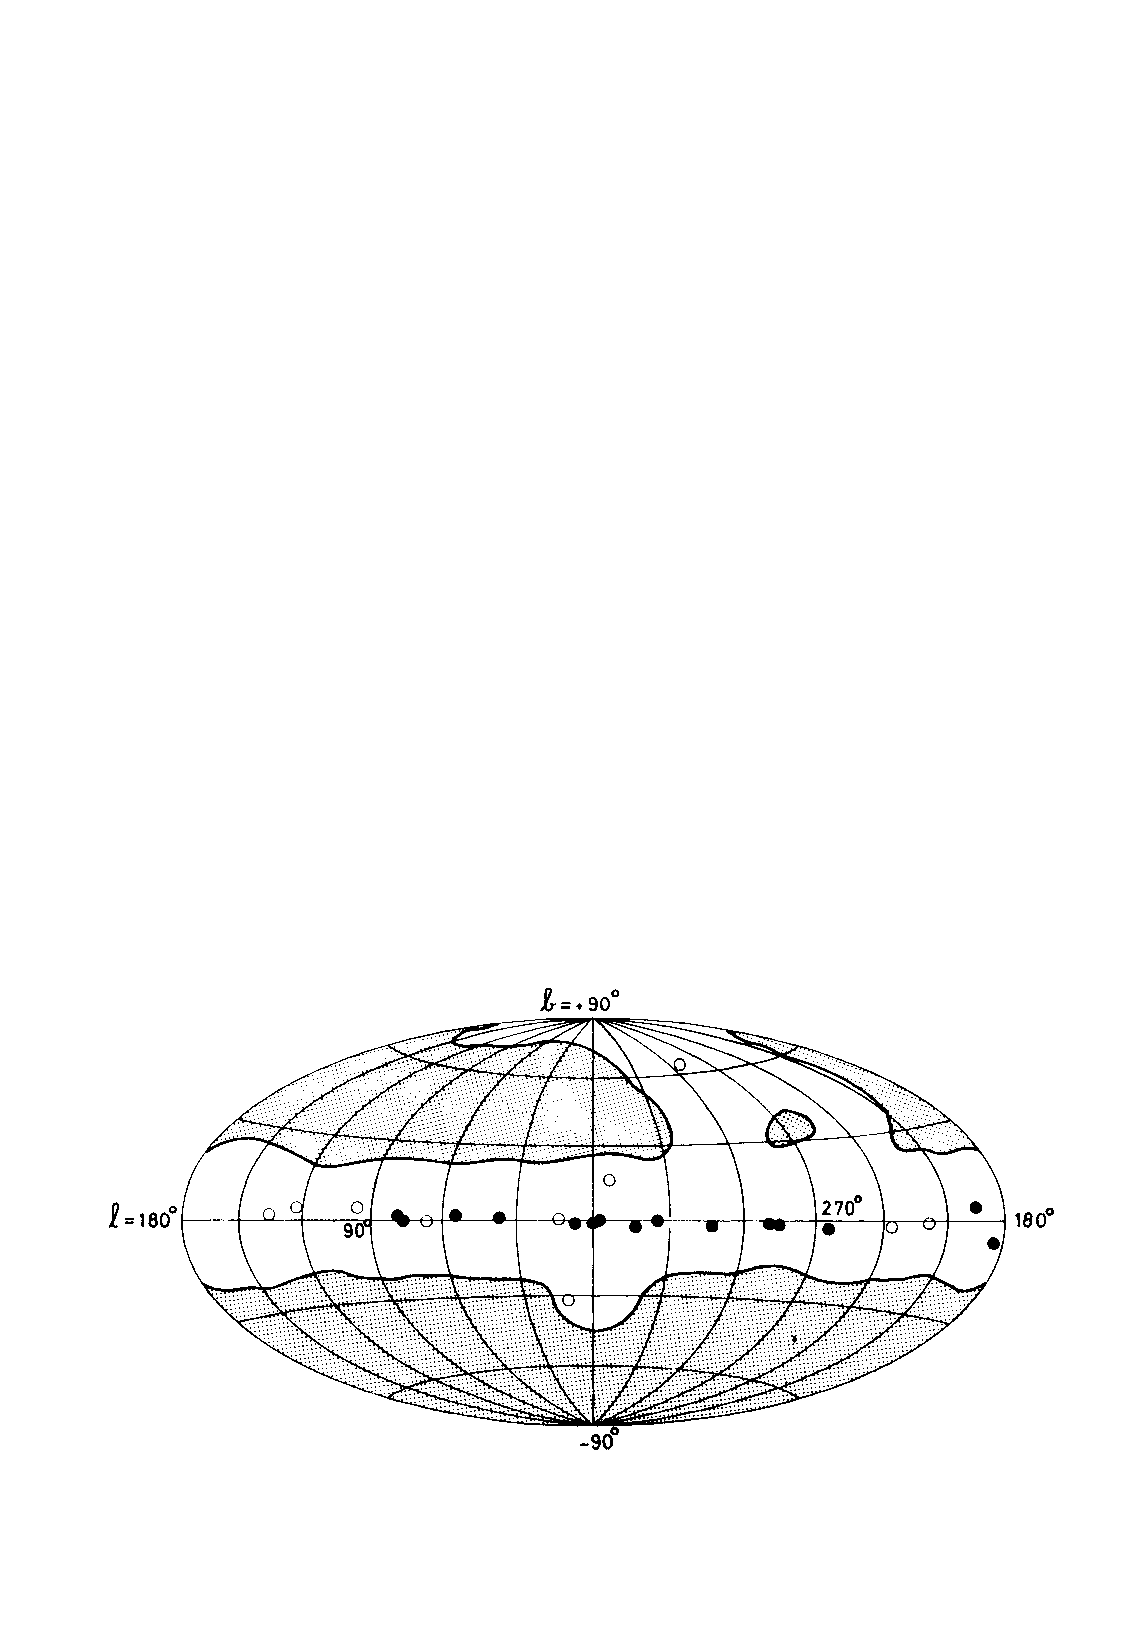
\includegraphics[width=\textwidth]{chapters/introduction/figures/cos_b_2nd_catalog.pdf}
  \figlabel{cos_b_skymap}
  \caption{
  A map of the sources observed by \cosb. The filled circles
  represent brighter sources. The unshaded region corresponds to
  the parts of the sky observed by \cosb.  This figure is from
  \cite{swanenburg_1981_second-catalog}.
  }
\end{figure}

The next major $\gamma$-ray experiment was \ac{EGRET},
launched
on board \ac{CGRO} in 1991. \ac{EGRET} had a design
similar to \ac{SAS-2}, but had an expanded energy range, operating from
$20\unitspace\mev$ to $30\unitspace\gev$, an improved effective area of
$\sim1500\unitspace\cm^2$ from $\sim500\mev$ to $\sim1\unitspace\gev$,
and an improved angular resolution, decreasing to $\sim0.5\degree$
at its highest energies \citep{thompson_1993a_calibration-energetic}.
At the time, \ac{CGRO} was the heaviest astrophysical experiment
launched into orbit, weighting $\sim17,000\unitspace\kg$. \ac{EGRET}
contributed $\sim6,000\unitspace\kg$ to the mass of \ac{CGRO}.
\figref{egret_detector} shows a schematic diagram of \ac{EGRET}.

\begin{figure}[htbp]
\centering
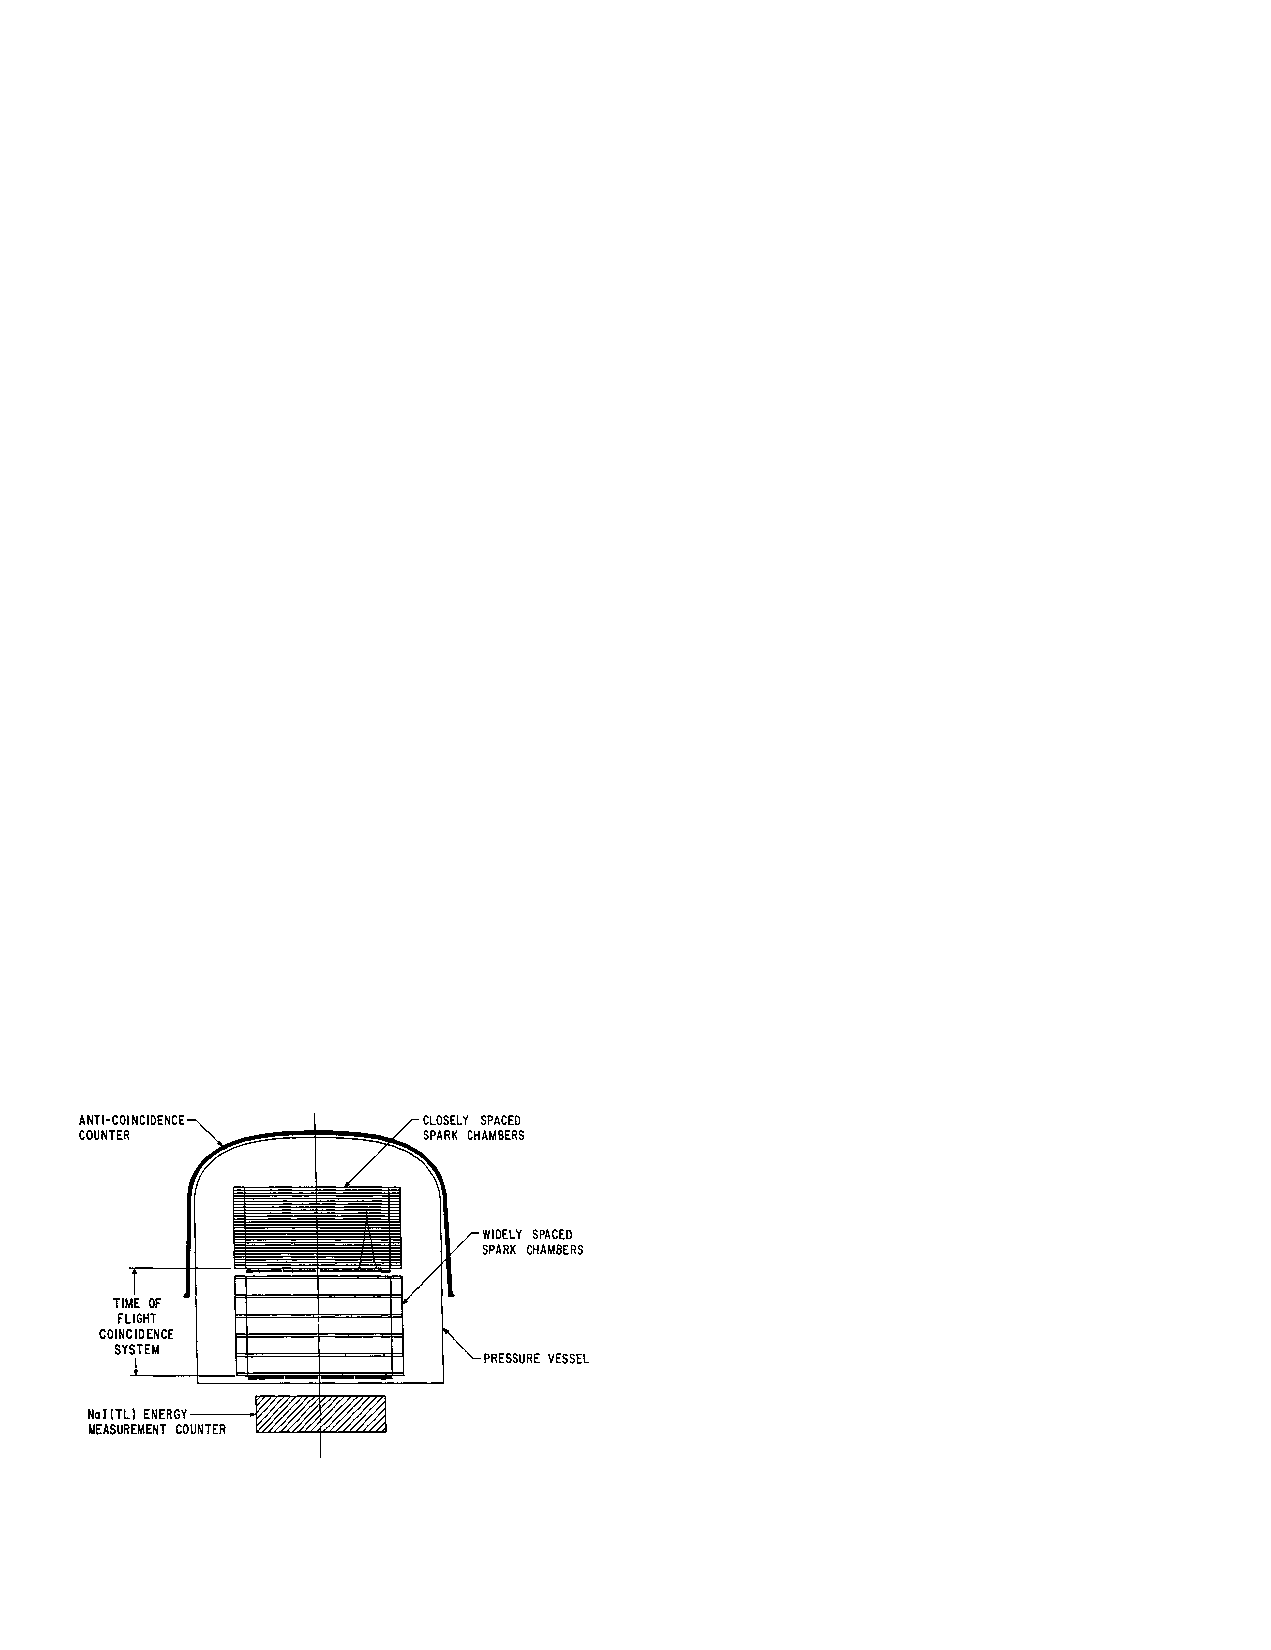
\includegraphics{chapters/introduction/figures/egret_detector.pdf}
\figlabel{egret_detector}
\caption{A diagram of the \ac{EGRET} detector.  This figure is from
\citep{thompson_1993a_calibration-energetic}.}
\end{figure}

\ac{EGRET} vastly expanded the field of $\gamma$-ray astronomy.
\ac{EGRET} detected six pulsars \citep{nolan_1996a_egret-observations} and
also the Crab Nebula \citep{nolan_1993a_observations-pulsar}.  \ac{EGRET}
also detected the LMC, the first normal galaxy outside of our galaxy to be
detected at $\gamma$-rays \citep{sreekumar_1992a_observations-large}.
\ac{EGRET} also detected Centarus A, the first radio galaxy
detected at $\gamma$-rays \citep{sreekumar_1999a_emission-nearby}.
In total, EGRET detected 271 $\gamma$-ray sources in \ac{3EG}
\citep{hartman_1999a_third-egret}. This catalog included 66
high confidence blazar identifications and 27 low-confidence AGN
identifications. \figref{third_egret_catalog_sources} plots the sources
observed by \ac{EGRET}.  In total, \ac{EGRET} detected over 1,500,000
celestial gamma rays \citep{thompson_2008a_gamma-astrophysics:}.

\begin{figure}[htbp]
\centering
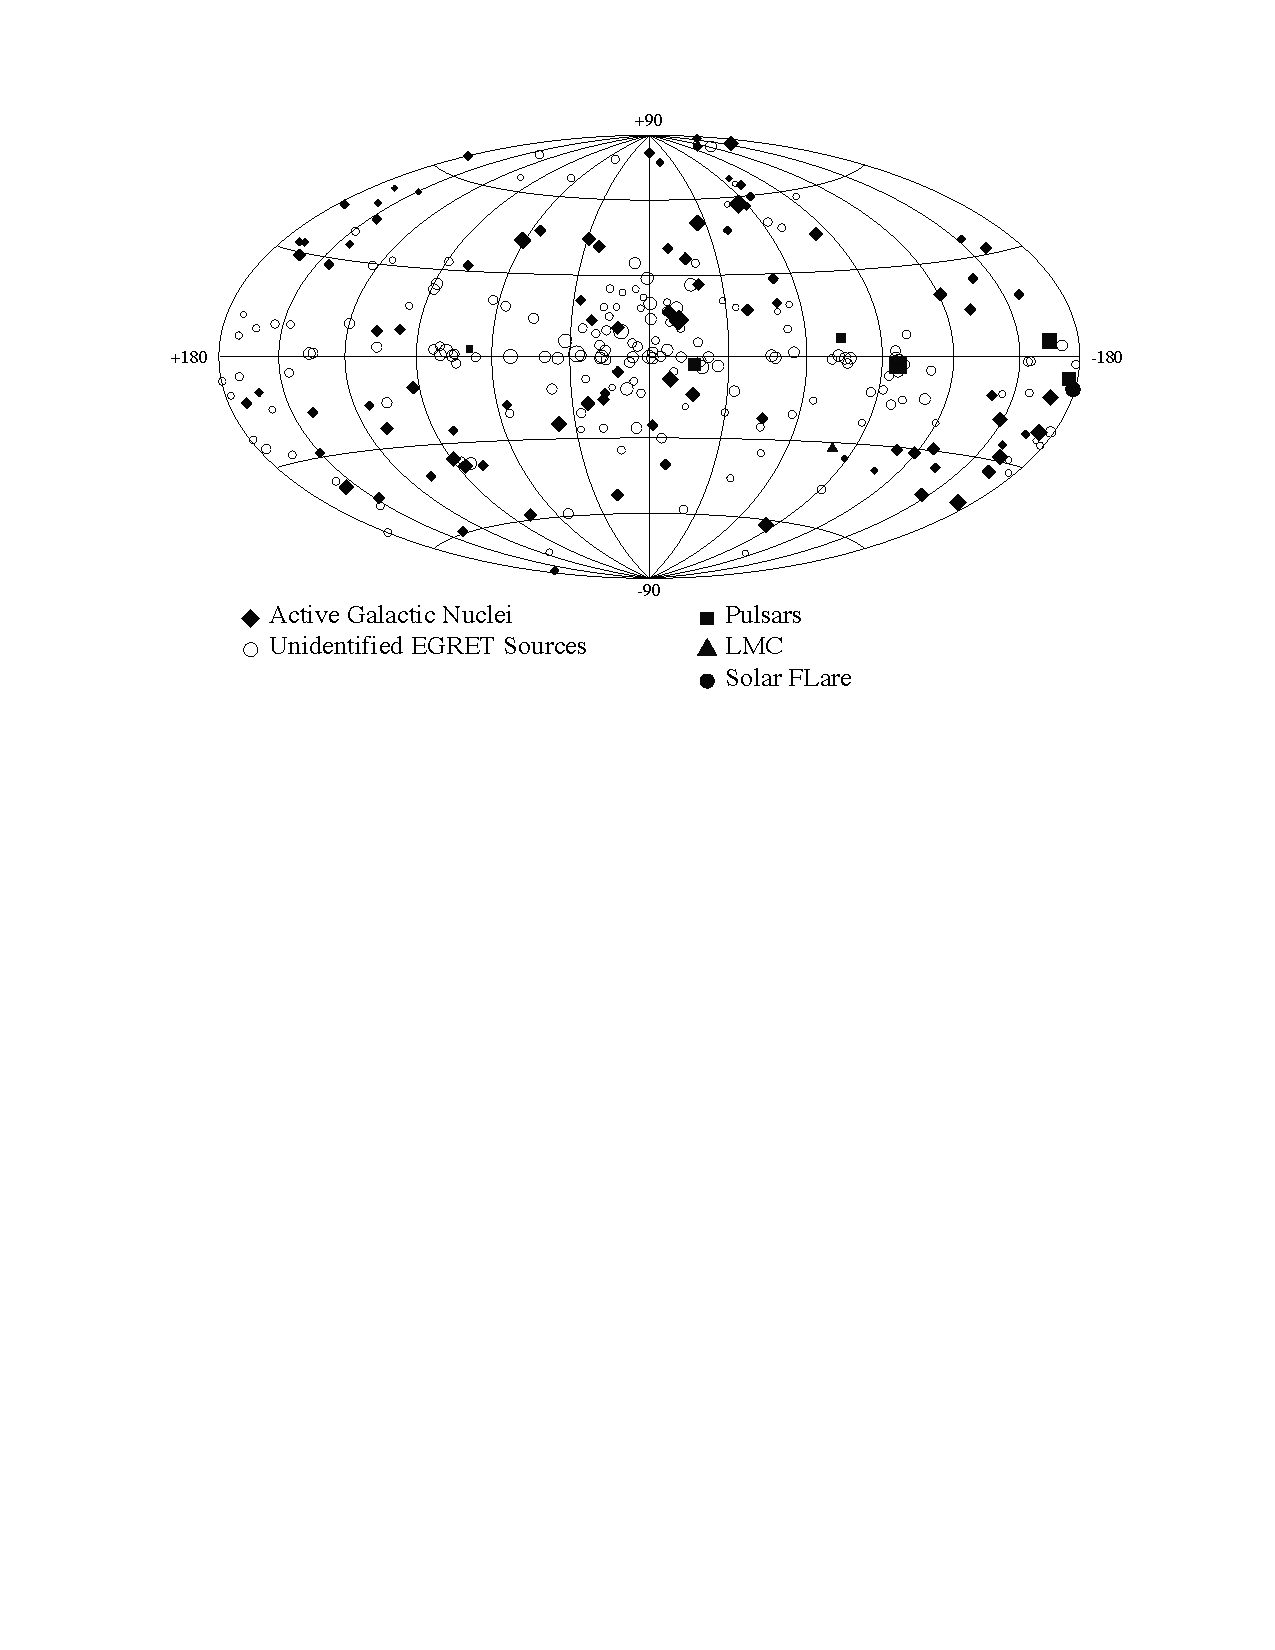
\includegraphics{chapters/introduction/figures/third_egret_catalog_sources.pdf}
\figlabel{third_egret_catalog_sources}
\caption{The position of \ac{EGRET} sources in the sky in galactic
coordinates.  The size of the source markers corresponds to the overall
source intensity.  This figure is from \citep{hartman_1999a_third-egret}.}
\end{figure}

Following \ac{EGRET}, the next major $\gamma$-ray observatories
were \ac{AGILE} \citep{pittori_2003a_gamma-ray-imaging}
and the \fermi Gamma-ray Space Telescope \citep{atwood_2009a_large-telescope}.  \ac{AGILE}
was an \ac{ASI} experiment launched in 2007 and \fermi was
a joint \ac{NASA} and \ac{DOE} experiment which was launched
in 2008.  The major difference between \ac{AGILE} and \fermi
was that \fermi has a significantly-improved effective area
\citep[$9,500\unitspace\cm^2$,][]{atwood_2009a_large-telescope}
compared to \ac{AGILE}
\citep[$\sim500\unitspace\cm^2$,][]{pittori_2003a_gamma-ray-imaging}.
We will discuss the \fermi detector in \secref{fermi_telescope}.
